\textbf{MiE. Microeconomía Avanzada. Curso 2023/2024. Entrega Febrero}
\begin{center}
    \textbf{Paredes Aguilera Christian Limbert}
\end{center}
\begin{center}
	\rule{1\textwidth}{0.4pt}
\end{center}

\begin{enumerate}[\textbf{Ejercicio} 1]

    % Ejercicio 1
    \item Considere una economía de intercambio con dos consumidores, $A$ y $B$, y dos mercancías, $x$ e $y$. Las dotaciones iniciales de los consumidores son $(x_A, y_A) = (15, 3)$ y $(x_B, y_B) = (5, 17)$. Las preferencias de los consumidores vienen representadas por las siguientes funciones de utilidad: $U_A(x, y) = x_Ay_A$ y $U_B(x, y) = x^2_By_B$. Defina, calcule y dibuje en una caja de Edgeworth el conjunto de asignaciones Pareto eficientes.\\

	Solución: Dado las dotaciones iniciales $(x_A,y_A)=(15,3)$, se tiene
	$$U_A=15*3=45.$$
	De donde, para $U_A=x_Ay_A$. Obtenemos,
	$$y_A=\frac{45}{x_A}.$$

	Luego, para $U_B=x^2_By_B$, se tiene
	$$U_B=x^2_By_B=5^2*17=425.$$
	De donde, para $U_B=x^2_By_B$. Obtenemos,
	$$y_B=\frac{425}{x^2_B}.$$

	\begin{center}
	    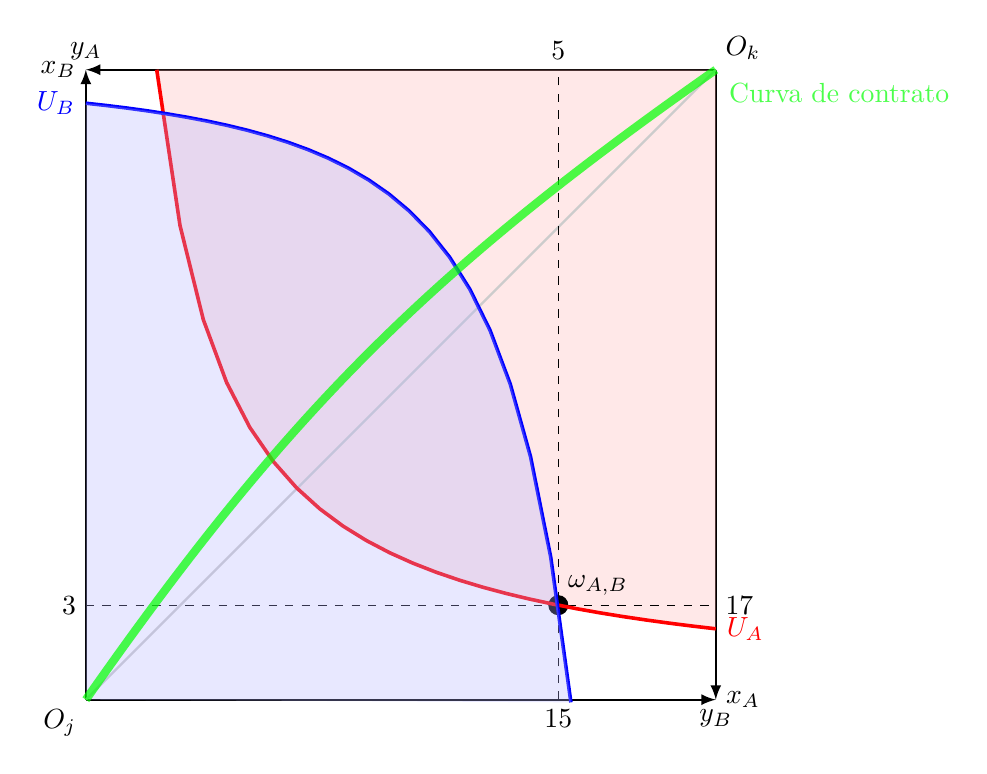
\begin{tikzpicture}[scale=0.4]
		\coordinate (A) at (0,0);
		\coordinate (B) at (20,20);
		\begin{scope}[->,>=latex,thick]
		    \draw (A) -- +(20,0)node[right]{$x_A$};
		    \draw (A) -- +(0,20)node[above]{$y_A$};
		    \draw (B) -- +(-20,0)node[left]{$x_B$};
		    \draw (B) -- +(0,-20)node[below]{$y_B$};
		\end{scope}
		\node[below left] at (A) {$O_j$};
		\node[above right] at (B) {$O_k$};

		\fill[fill=red!30,opacity=.3] (3,20) -- plot[domain=2.25:20] (\x,{(45/\x}) -- (20,20) -- cycle;

		\draw[fill=black] (15,3) circle (0.3cm) node[above right]{$\omega_{A,B}$};

		\draw[thick,gray!40] (0,0) -- (20,20);

		\draw[dashed] (0,3)node[left]{$3$} -- (20,3)node[right]{$17$};
		\draw[dashed] (15,0)node[below]{$15$} -- (15,20)node[above]{$5$};

		\draw[variable=\x,domain=2.25:20,thick,red,line width=1.3pt] plot ({\x},{45/\x})node[right]{$U_A$};

		\begin{scope}[rotate around={180:(10,10)}]  % Rotate around point A
		\draw[variable=\x,domain=4.6:20,thick,blue,line width=1.3pt] plot ({\x},{425/(\x^2)})node[left]{$U_B$};
		\fill[fill=blue!30,opacity=.3] plot[domain=4.6:20] (\x,{(425/\x^2}) -- (20,20) -- cycle;
		\end{scope}

		\draw[thick,green,line width=3pt,opacity=.7] (0,0) to[out=55,in=215] (20,20)node[below right]{Curva de contrato};

	    \end{tikzpicture}
	\end{center}
	\vspace{.5cm}

    % Ejercicio 2
    \item Considere una economía con dos bienes, trabajo y consumo, y una SOF que aplica el criterio del $maximin$ a la siguiente medida comparable de utilidad. Para todo $i \in N, s_i \in S, z_i \in Z$ y $R_i \in \mathcal{R}$:
	$$u_k(z_i , s_i , R_i) = u \Leftrightarrow z_i I_i \max |_{R_i} B(s_i ,(k, u)).$$ 
	Esta medida se construye de la siguiente manera. Para cada individuo $i \in N$ se define primero, usando su habilidad si, el conjunto presupuestario más pequeño que le permite alcanzar la misma utilidad que con su cesta $z_i$. A continuación, la medida de utilidad comparable se construye como la cantidad de consumo que podría alcanzar escogiendo en este conjunto una cantidad de trabajo $k$. Así, en el ejemplo adjunto los 4 individuos están asociados con exactamente el mismo nivel comparable de utilidad cuando la cantidad de trabajo de referencia es $k = 0.5$. \\

	Partiendo de este mismo ejemplo, orden de las utilidades comparables de estos mismos 4 agentes cuando $k = 0.4$. ¿Cuál sería el orden si $k = 0.6$? ¿Qué causa la diferencia entre estas dos ordenaciones? \\

	¿Cuál sería la ordenación social entre las asignaciones $(z_1, z_3)$ y $(z_4, z_2)$ si utilizásemos una SOF basada en esta medida de bienestar? ¿Y si utilizasemos la SOF $\textbf{R}^{slex}$?\\

	Solución: Para ordenar las utilidades comparables de los cuatro agentes cuando $k = 0.4$, necesitamos analizar cómo se desplazarían las restricciones presupuestarias al reducir la cantidad de trabajo de $0.5$ a $0.4$. A menor cantidad de trabajo, cada agente tendría una capacidad menor para generar ingresos, lo que a su vez reduciría su conjunto presupuestario. Esto se traduce en que las curvas de restricciones presupuestarias se desplazarían hacia la izquierda en el gráfico. La utilidad comparable se mide por el nivel de consumo que pueden alcanzar con ese menor nivel de trabajo. Ahora, aquellos con restricciones presupuestarias más inclinadas hacia el eje del consumo (indicando una mayor eficiencia en la transformación de trabajo en consumo) tendrán utilidades comparables más altas, ya que podrán alcanzar niveles más altos de consumo incluso con menos trabajo.

	Por lo tanto, el orden de las utilidades comparables de esos agentes sera:
	$$z_1 \succ z_2 \succ z_3 \succ z_4.$$

	Por otro lado, si $k = 0.6$, estaríamos aumentando la cantidad de trabajo desde el nivel de referencia de $0.5$. Esto ampliaría las posibilidades presupuestarias de los agentes, desplazando las curvas de restricciones presupuestarias hacia la derecha. Los agentes con curvas más inclinadas hacia el eje del consumo se beneficiarían proporcionalmente más de este aumento en el trabajo, ya que pueden convertir el trabajo extra en un mayor consumo.

	Por lo tanto, el orden de las utilidades comparables de esos agentes sera:
	$$z_4 \succ z_3 \succ z_2 \succ z_1.$$

	La diferencia entre las dos ordenaciones ($k = 0.4$ y $k = 0.6$) se debe a cómo cada agente convierte el trabajo en consumo. Algunos agentes pueden ser más eficientes en convertir trabajo adicional en consumo (tienen una mayor tasa marginal de transformación), por lo que un cambio en la cantidad de trabajo tiene un efecto desproporcionado en su utilidad comparable. Por lo tanto, las diferencias en las inclinaciones de las restricciones presupuestarias entre los agentes pueden llevar a diferentes reordenamientos de las utilidades comparables cuando se cambia la cantidad de trabajo referencial.\\

	Luego, la ordenación social entre las asignaciones $(z_1, z_3)$ y $(z_4, z_2)$ si utilizásemos una SOF basada en esta medida de bienestar sería:
	$$(z_1,z_3)P(e) (z_4,z_2).$$
	Lo que significa que la sociedad prefiere estrictamente la asignación $(z_1,z_3)$ a la asignación $(z_4,z_2)$.

	Para la SOF $\textbf{R}^{slex}$, la ordenación social entre las asignaciones $(z_1, z_3)$ y $(z_4, z_2)$ sería:
	$$(z_1,z_3)R^{e} (z_4,z_2).$$
	Lo que significa que la sociedad considera que la asignación $(z_1,z_3)$ es al menos tan buena como la asignación $(z_4,z_2)$.\\\\


    % Ejercicio 3
    \item  Considere una economía que consta de tres individuos que tienen unas demandas legítimas de $c_1 = 4$, $c_2 = 16$ y $c_3 = 20$. Calcule, para las siguientes 5 reglas, las soluciones de reparto para cada una de las cinco posibles dotaciones iniciales propuestas (ver tabla).

	\begin{center}
	    \begin{tabular}{|l|c|c|c|c|c|c|}
		\hline
		& P & CEA & CEL & CE & CD & SP$^{1\succ 2}$\\
		\hline
		E = 10 & (1, 4, 5) & (4, 3, 3) & (0, 6, 4) & (4, 3, 3) & (0, 6, 4) & (4, 6, 0) \\
		E = 15 & (1.5, 6, 7.5) & (4, 5.5, 5.5) & (0, 8, 7) & (4, 5.5, 5.5) & (0, 7.5, 7.5) & (4, 11, 0) \\
		E = 20 & (2, 8, 10) & (4, 8, 8) & (0, 10, 10) & (4, 8, 8) & (0, 10, 10) & (4, 16, 0) \\
		E = 30 & (3, 12, 15) & (4, 13, 13) & (0, 16, 14) & (4, 13, 13) & (0, 15, 15) & (4, 26, 0) \\
		E = 38 & (3.8, 15.2, 19) & (4, 17, 17) & (0, 18, 20) & (4, 17, 17) & (0, 19, 19) & (4, 34, 0) \\
		\hline
	    \end{tabular}
	\end{center}
	\vspace{.5cm}

    % Ejercicio 4
    \item Demuestre gráficamente (como se hizo en las notas de clase) las siguientes incompatibilidades entre reglas de asignación y propiedades:

	\begin{enumerate}[(a)]

	    % a)
	    \item Prioridad Secuencial (SP) y Progresividad (PROG). 

		Solución:
		\begin{center}
		    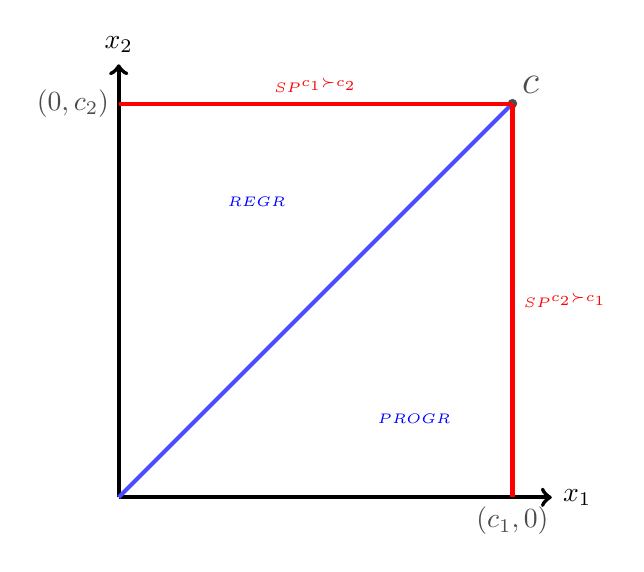
\begin{tikzpicture}[scale=.5]
			% Ejes
			\draw[->,line width = 1.5pt] (0,0) -- (11,0) node[right] {$x_1$};
			\draw[->,line width = 1.5pt] (0,0) -- (0,11) node[above] {$x_2$};

			\draw[fill,black!70](0,10)node[left]{$(0,c_2)$} -- (10,10)circle(3pt)node[above right]{\Large$c$} -- (10,0)node[below]{$(c_1,0)$};


			\draw[blue!70,line width = 1.5pt](0,0) -- (10,10);

			\draw[blue,line width = 1.5pt](3.5,7.5)node[]{\tiny$REGR$};
			\draw[blue,line width = 1.5pt](7.5,2)node[]{\tiny$PROGR$};

			\draw[red,line width = 1.5pt](10,0)node[right,yshift=2.5cm]{\tiny$SP^{c_2\succ c_1}$} -- (10,10);

			\draw[red,line width = 1.5pt](0,10)node[above,xshift=2.5cm]{\tiny$SP^{c_1 \succ c_2}$} -- (10,10);

		    \end{tikzpicture}
		\end{center}
		\vspace{.5cm}


	    % b)
	    \item Igual Ganancia Restringida (CEA y Regresividad (REGR). 

		Solución:
		\begin{center}
		    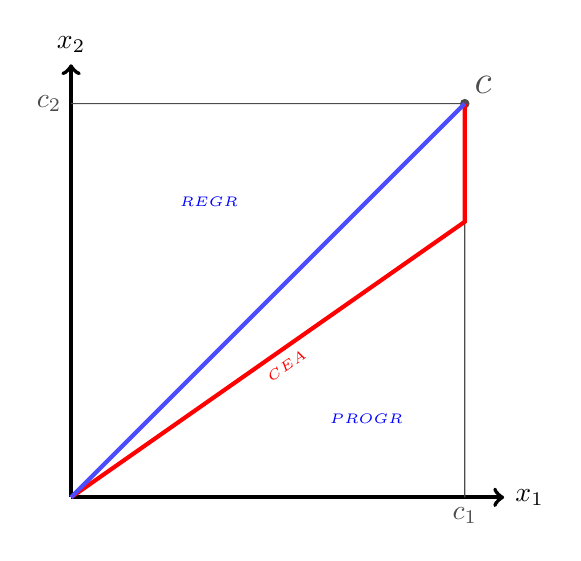
\begin{tikzpicture}[scale=.5]
			% Ejes
			\draw[->,line width = 1.5pt] (0,0) -- (11,0) node[right] {$x_1$};
			\draw[->,line width = 1.5pt] (0,0) -- (0,11) node[above] {$x_2$};

			\draw[fill,black!70](0,10)node[left]{$c_2$} -- (10,10)circle(3pt)node[above right]{\Large$c$} -- (10,0)node[below]{$c_1$};

			\draw[red,line width = 1.5pt](0,0)node[below,rotate=35,xshift=3.2cm]{\tiny$CEA$} -- (10,7) -- (10,10);

			\draw[blue!70,line width = 1.5pt](0,0) -- (10,10);

			\draw[blue,line width = 1.5pt](3.5,7.5)node[]{\tiny$REGR$};
			\draw[blue,line width = 1.5pt](7.5,2)node[]{\tiny$PROGR$};

		    \end{tikzpicture}
		\end{center}
		\vspace{.5cm}

	    % c)
	    \item Igual Pérdida Restringida (CEL) y Punto Medio (MIDPOINT).

		Solución:
		\begin{center}
		    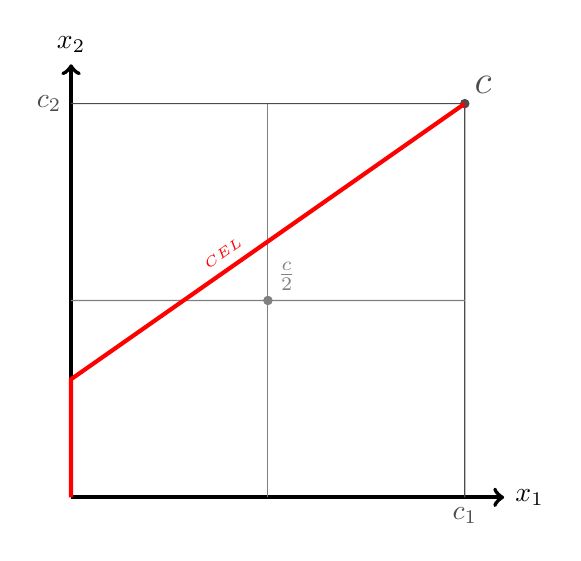
\begin{tikzpicture}[scale=.5]
			% Ejes
			\draw[->,line width = 1.5pt] (0,0) -- (11,0) node[right] {$x_1$};
			\draw[->,line width = 1.5pt] (0,0) -- (0,11) node[above] {$x_2$};

			\draw[fill,black!70](0,10)node[left]{$c_2$} -- (10,10)circle(3pt)node[above right]{\Large$c$} -- (10,0)node[below]{$c_1$};

			\draw[fill,gray] (0,5) -- (5,5) circle (3pt) node[above right]{$\frac{c}{2}$} -- (10,5);
			\draw[fill,gray] (5,0) -- (5,10);

			\draw[red,line width = 1.5pt](0,0) -- (0,3)node[above,rotate=35,xshift=2.5cm]{\tiny$CEL$} -- (10,10);

		    \end{tikzpicture}
		\end{center}
		\vspace{.5cm}

	    % d)
	    \item Igualitaria Restringida (CE) y Derechos Mínimos Primero (MINRIGHFI).

		Solución:
		\begin{center}
		    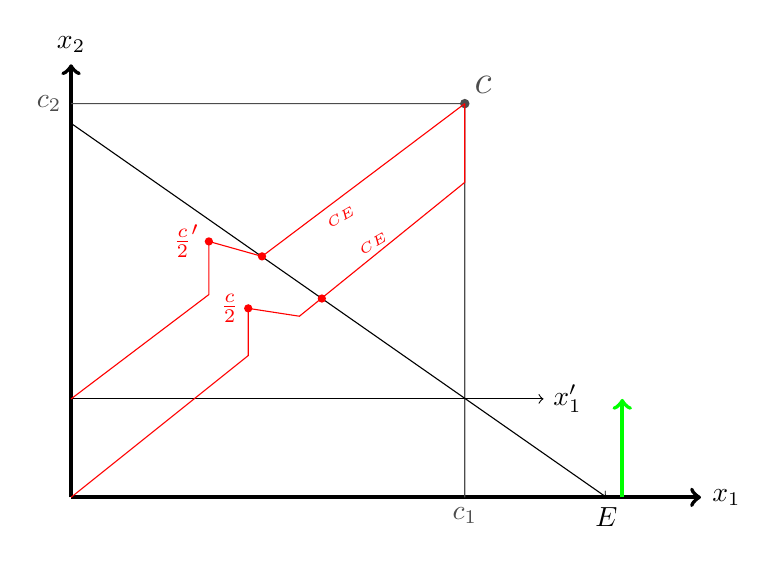
\begin{tikzpicture}[scale=.5]
			% Ejes
			\draw[->,line width = 1.5pt] (0,0) -- (16,0) node[right] {$x_1$};
			\draw[->,line width = 1.5pt] (0,0) -- (0,11) node[above] {$x_2$};

			\draw[fill,black!70](0,10)node[left]{$c_2$} -- (10,10)circle(3pt)node[above right]{\Large$c$} -- (10,0)node[below]{$c_1$};

			\draw[->](0,2.5) -- (12,2.5)node[right]{$x_1'$};

			\draw[->](0,9.5) -- (13.6,0)node[below]{$E$};

			\draw[red](0,0) -- (4.5,3.6) -- (4.5,4.8) -- (5.8,4.6) -- (10,8) -- (10,10);
			\fill[red](4.5,4.8)circle(3pt)node[left]{$\frac{c}{2}$};

			% desplazamiento
			\draw[red](0,2.5) -- (3.5,5.15) -- (3.5,6.5) -- (4.85,6.12)node[xshift=1cm,yshift=.5cm,rotate=30]{\tiny$CE$} -- (10,10);
			\fill[red] (3.5,6.5)circle(3pt)node[left]{$\frac{c}{2}'$};
			\fill[red](4.85,6.12)circle(3pt)node[xshift=1.5cm,rotate=30,above]{\tiny$CE$};

			\fill[red](6.37,5.05)circle(3pt);

			\draw[->,line width=1.5pt,green](14,0)--(14,2.5);

		    \end{tikzpicture}
		\end{center}

	\end{enumerate}


\end{enumerate}
